\section{Durchführung}
\label{sec:Durchführung}
\subsection{Versuchsaufbau}
Der Versuchsaufbau besteht aus einer Kupferröntgenröhre, welche mit $\SI{35}{\kilo\volt}$ betrieben wird.
Diese strahlt auf eine Konstruktion welche einen LiF-Kristall oder ein Plexiglas-Streuer hält.
Die Konstruktion kann mit einem gewünschtem Winkel gegenüber der Röntgenröhre ausgerichtet werden, sodass die eingespannten Materiallien mit unterschiedlichen Winkeln bestrahlt werden können.
An der Halterung für die Materiallien ist zudem ein Geiger-Müller-Zählrohr befestigt.
Dieses wird so befestigt, dass der Einfallswinkel des Strahls der Röntgenröhre auf das Materiall, gleich dem Ausfallswinkel des reflektierten Strahls ist.
Der fertige Versuchsaufbau ist in der Abbildung \ref{fig:aufbau} zu sehen.
Die Abbildung wurde aus der Versuchsanleitung \cite{anleitung} entnommen.

\begin{figure}
    \centering
    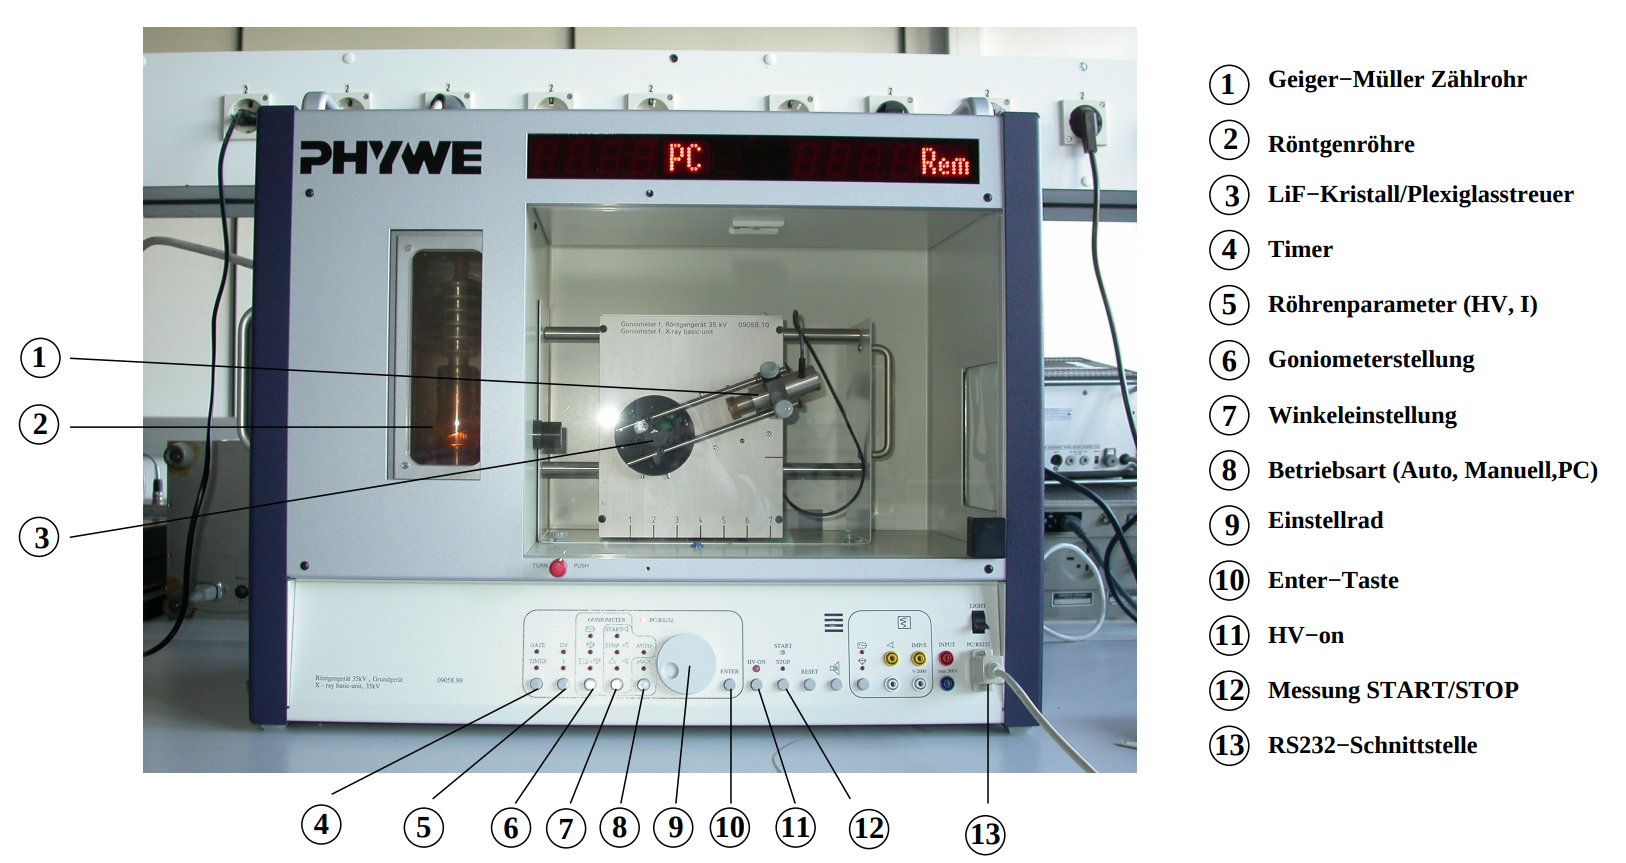
\includegraphics[width=\textwidth]{content/data/Roehre.png}
    \caption{Der fertige Versuchsaufbau, mit der Röhre links im Bild und dem Zählrohr rechts.}
    \label{fig:aufbau}
\end{figure}

\subsection{Versuchsablauf}
Zur Bestimmung des Spektrums der Röntgenröhre wird zunächst der LiF-Kristall in der vorgesehenden Halterung befestigt.
Nun wird der Winkel zwischen der Strahlung und der Halterung auf $8 \si{\degree}$ gestellt.
Für diesen Teil des Versuchs muss eine $2 \si{\milli\meter}$ Blende an der Röntgenröhre verwendet werden.
Danach wird die Röntgenröhre unter Spannung gestellt und die Werte, welche das Geiger-Müller-Zählrohr nach $5\si{\second}$ - $10\si{\second}$ anzeigt, notiert.
Nun wird der Winkel um $\SI{0.2}{\degree}$ erhöht und die Messung erneut durchgeführt.
Der Winkel muss so lange erhöht werden bis dieser einen Wert von $\SI{25}{\degree}$ erreicht hat.
\\\\
Nun wird ein Aluminium-Absorber zwischen der Röntgenröhre und den Kristall befestigt.
Der Winkel zwischen Kristallhalterung und Röntgenröhre muss auf $7\si{\degree}$ eingestellt werden.
Konträr zu dem vorherigem Aufbau, wird nun nach einer Messzeit von $200 \si{\second}$ der Wert des Geiger-Müller-Zählrohr notiert und der Winkel nur um $\SI{0.1}{\degree}$ erhöht.
Der Winkel wird bis zu einem Wert von $10\si{\degree}$ erhöht.
Nachdem alle Werte notiert wurden, wird der selbe Ablauf einmal ohne Aluminium-Absorber wiederholt.
\\\\
Zur Bestimmung der Comptonwellenlänge wird nun der LiF-Kristall durch ein Plexiglas-Streuer ersetzt.
Die Halterung muss nun auf $45 \si{\degree}$ eingestellt werden, sodass der Geiger-Müller-Zähler einen Winkel von $90\si{\degree}$ zur Röntgenröhre hat.
Nun wird die Intensität $I_0$ der Röntgenröhre gemessen, die Messzeit beträgt dabei $300\si{\second}$.
Nach der Messung muss zwischen Röntgenröhre und Kristall der Aluminium Absorber eingesetzt werden, erneut wird die Intensität gemessen, diese wird $I_1$ betitelt.
Zuletzt wird der Absorber zwischen Kristall und Zählrohr eingesetzt und die Intensität $I_2$ gemessen.
